\chapter{Design}

\begin{longtabu} to \linewidth{@{}l l l X[j]@{}}
    Version &    Dato &    Ansvarlig &    Beskrivelse\\[-1ex]
    \midrule
    0.1 &	8/09 2015	&	Alle		& Oprettelse  af dokument\\
    0.2 &	27/10 2015 & SSK, NHL, FRM & Påbegyndelse af hardware design \\
    0.3 &	04/11 2015 & TSN, JTH, MFJ & Påbegyndelse af software design \\
    0.2 &	06/11 2015 & Alle & Første udkast til færdigt design afsnit \\
    0.3 & 	16/11 2015 & Alle & Review rettelser af design afsnittet \\
\label{version design}
\end{longtabu}


\section{Indledning}
Formålet med designafsnittet er at beskrive hardwaren og softwaren for blodtryksmålingssystemet. Systemet beskrives ved hjælp af udregninger, diagrammer, figurer og skitser som tydeliggør, hvordan de forskellige delelementers funktionalitet er, samt hvilke tanker der ligger til grund for den endelige implementering (se afsnit \ref{Hardware implementering} for hardware og afsnit \ref{implementering} for software).

\section{Hardware arkitektur}
I følgende afsnit beskrives blodtryksmålingssystemet og dets delkomponenters opbygning.
\\
\begin{figure}[H]
	\centering
	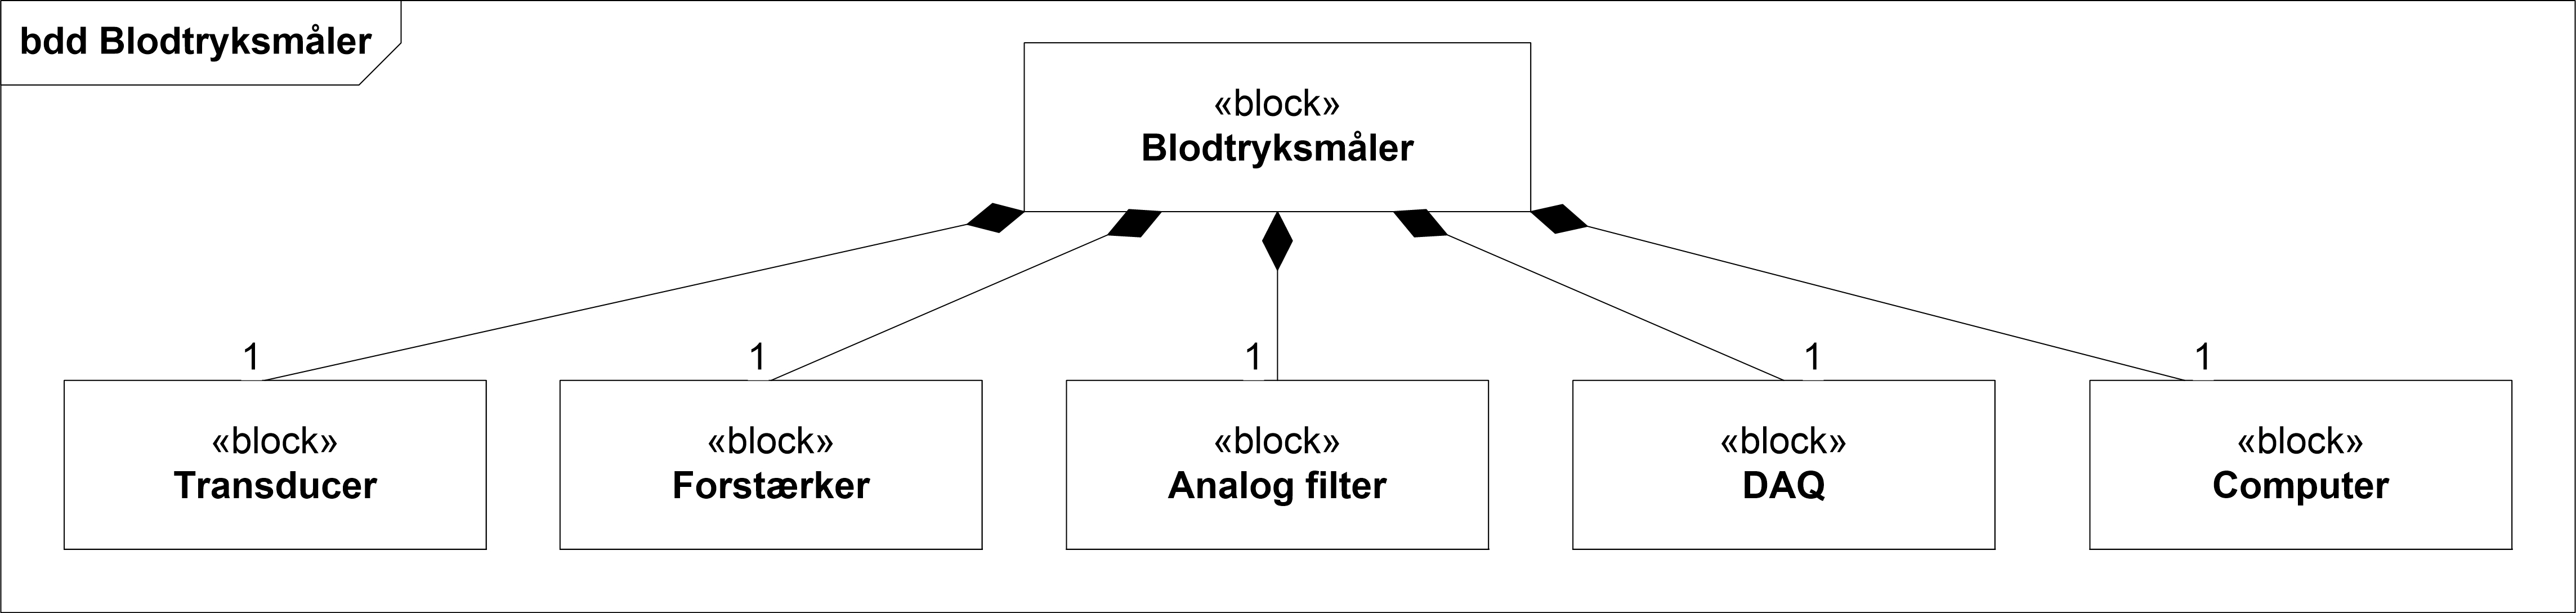
\includegraphics[width=1\textwidth]{Figurer/Hardware/BDD1}
	\caption{Blokdiagram for blodtryksmålingssystemet.}
	\label{BDD blodtryksmaaler}
\end{figure}

Ud af blokdiagrammet, figur \ref{BDD blodtryksmaaler}, kan man se, at blodtryksmålingssystemet består af en transducer, en forstærker, et analogt filter, en DAQ og en computer.\\
\begin{figure}[H]
	\centering
	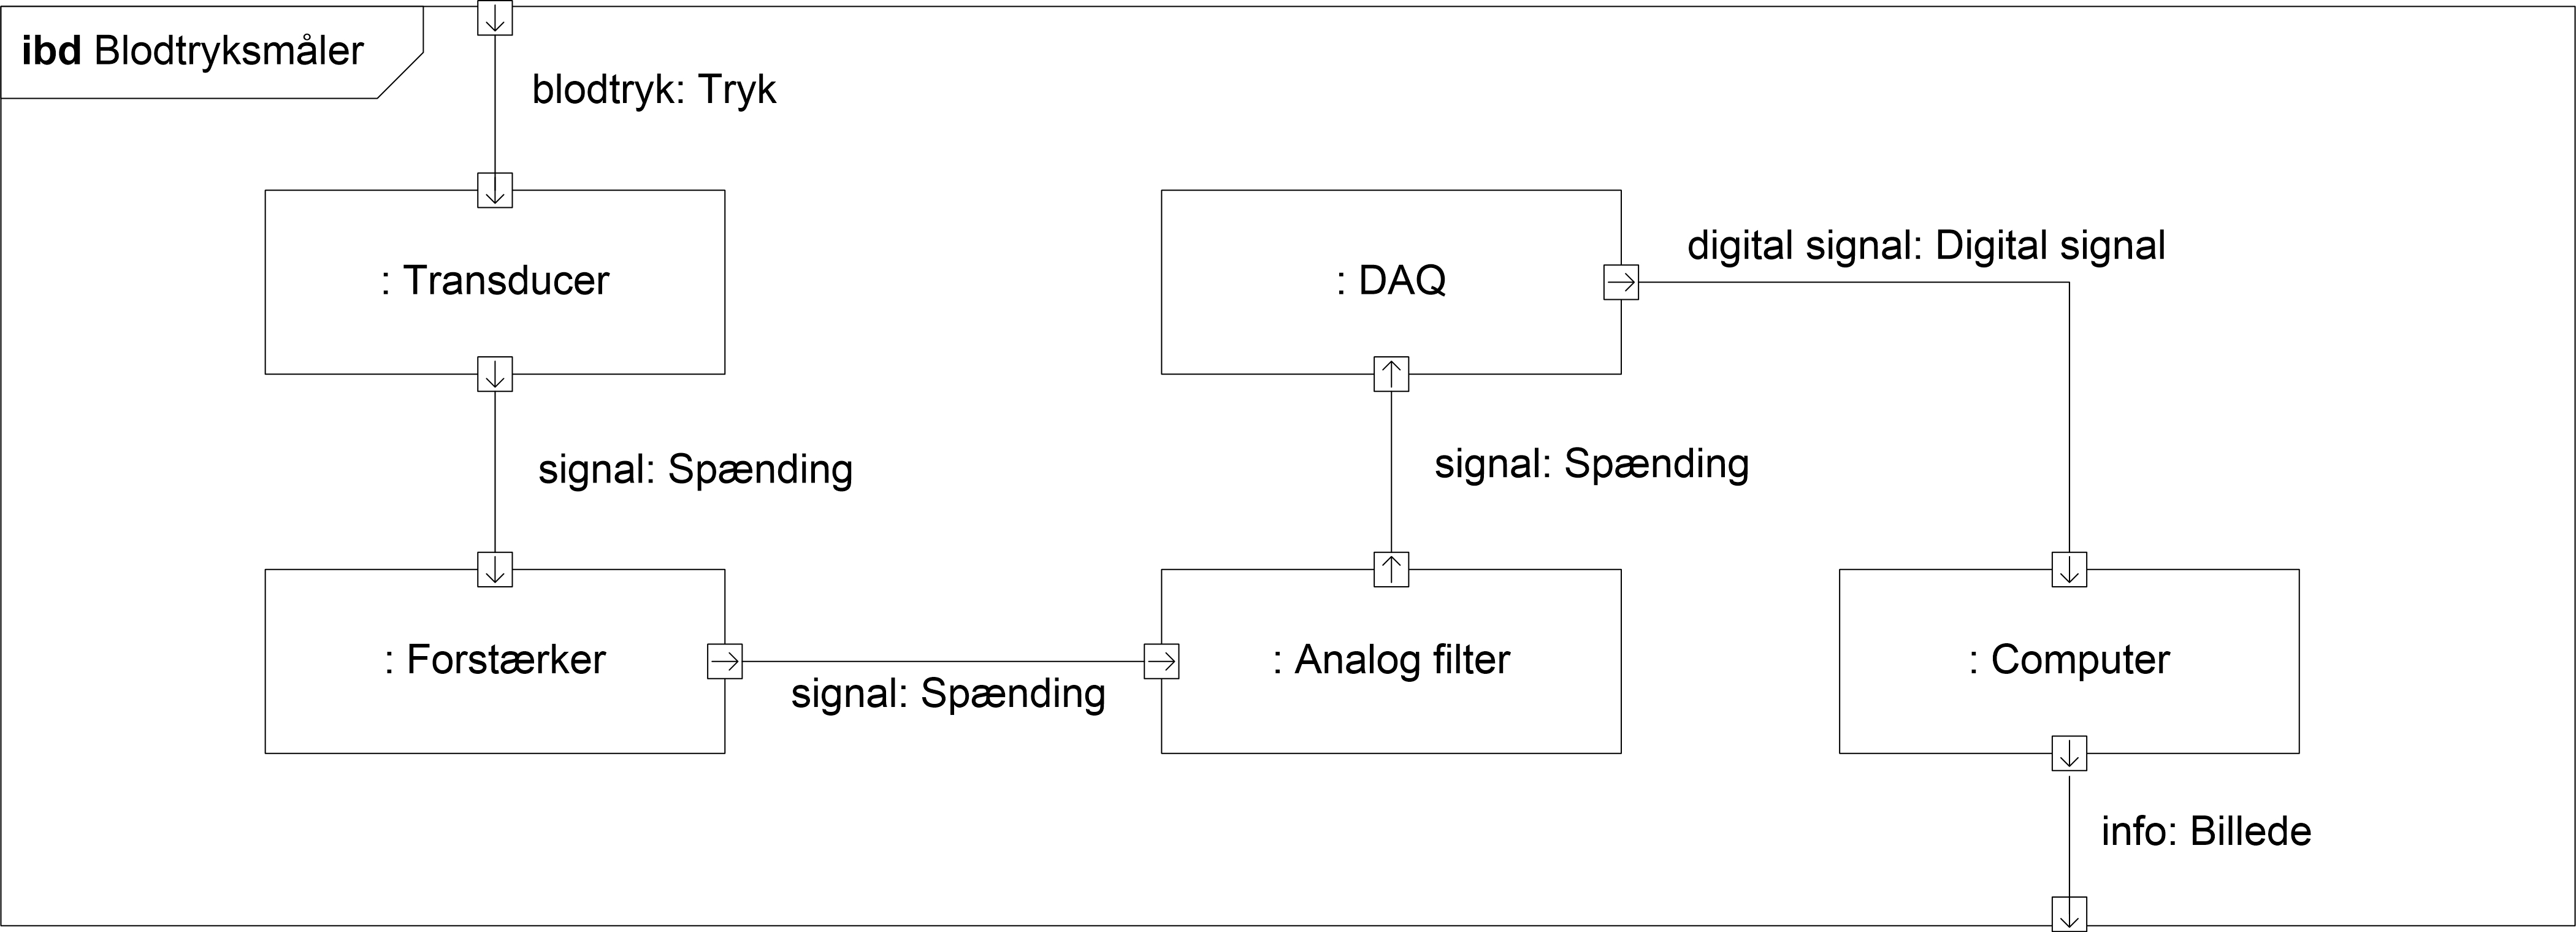
\includegraphics[width=1\textwidth]{Figurer/Hardware/IBD}
	\caption{Internt blokdiagram for blodtryksmålingssystemet.}
	\label{IBD blodtryksmaaler}
\end{figure}

Ud af det interne blokdiagram, figur \ref{IBD blodtryksmaaler}, kan det ses, at blodtrykket i form af det målte tryk kommer ind i transduceren. Transduceren, som omformer det målte tryk til et spændingssignal, sender signalet videre til forstærkeren. Fra forstærkeren sendes signalet over i det analoge filter og derfra ind i DAQ'en. Endeligt sendes det digitale signal fra DAQ'en over i en computer, der fortolker signalet som et billede, der vises til omverdenen.

\subsection{Design af forstærker}
Forstærkeren er designet med tanke på, at det er meget små spændinger, der arbejdes med. Grundet dette, er en almindelig operationsforstærker fravalgt, da dens reelle indgangsimpedans er for lav. En instrumentationsforstærkers indgangsimpedans i den virkelige verden er højere, og den kan dermed opfange meget små signaler som f.eks. blodtryk, der opererer i mV.\\
Vejleder rådede herefter til, at der skulle bruges instrumentationsforstærkeren INA114. Forstærkerens design er valgt ud fra instrumentationsforstærkerens datablads anbefalinger og kan ses på figur \ref{instrumentation}.\\ 
\begin{figure}[H]
	\centering
	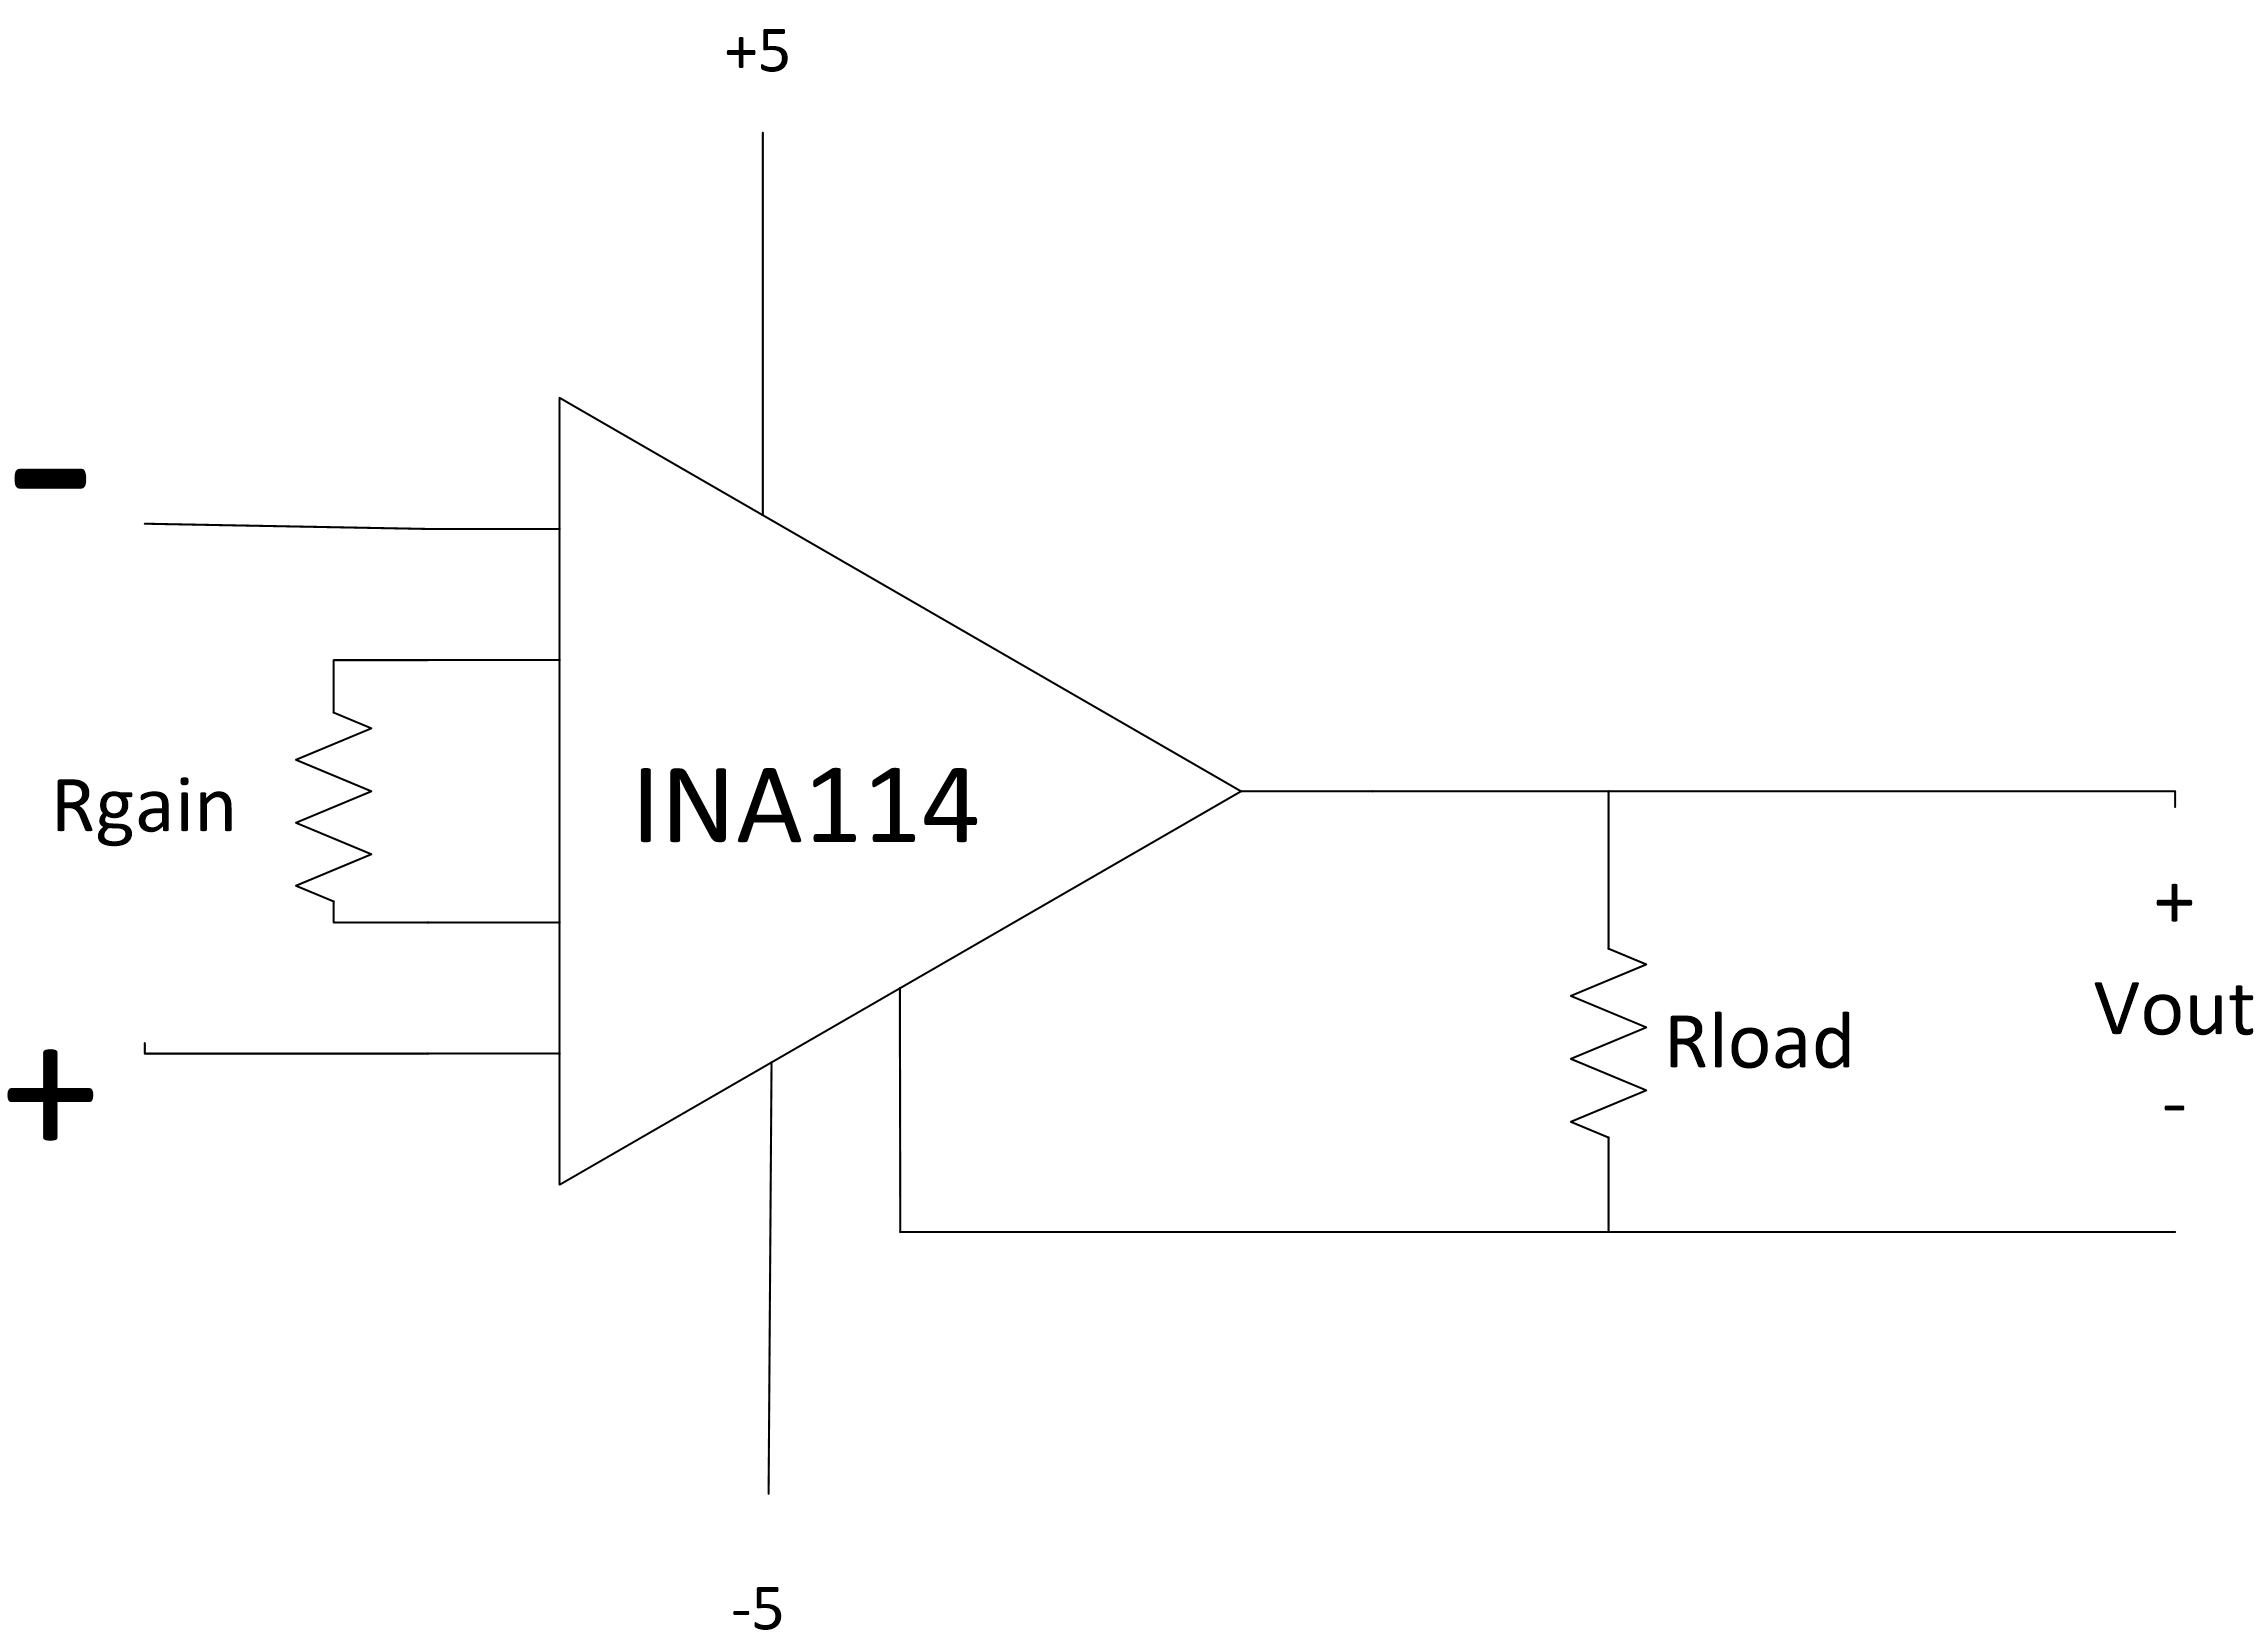
\includegraphics[width=0.6\textwidth]{Figurer/Hardware/Forstaerker}
	\caption{Det overordnede design af forstærkeren.}\label{instrumentation}
\end{figure}



$R_{gain}$ er modstanden, som bestemmer hvor meget forstærkning instrumentationsforstærkeren skal give og $R_{load}$ er den belastning, der kommer efter kredsløbet. I dette tilfælde er belastningen det analoge filter. For at finde $R_{gain}$’s størrelse, kræves viden om, hvor meget forstærkning, der er brug for. Dette findes ved at bestemme den maksimale spænding, som transduceren kan give i en blodtrykssituation. Dette regnestykke kan ses realiseret i ligning \ref{ligning1}:

\begin{align}
	VT_{max}=T_{max}\cdot V_{max}\cdot Hg_{max}=5\frac{\mu V}{V/mmHg}\cdot 5V\cdot 250mmHg=6,25mV
	\label{ligning1}
\end{align}

Spændingen ønskes skaleret op til DAQ’ens dynamikområde, som ligger omkring +/- 2,5V. Forstærkningsfaktoren udregnes ved simpel brøkregning, som ses på ligning \ref{ligning2}:

\begin{center}
	\begin{align}
		G=\frac{2,5}{6,25 \cdot 10^{-3}}=400
		\label{ligning2}
	\end{align}
\end{center}

INA114’s datablad giver en ligning for udregning af forstærkning. Da forstærkningen er kendt, omskrives ligning \ref{ligning3}, så modstanden $R_{gain}$’s værdi i stedet bestemmes:\\


\begin{align}
	Gain=1+\frac{50k\Omega}{R_{gain}}\to G-1=\frac{50k\Omega}{R_{gain}}\to \frac{50k\Omega}{G-1}=R_{gain}
	\label{ligning3}
\end{align}

Herefter kan den ohmske værdi af $R_{gain}$ bestemmes, hvilket sker i ligning \ref{ligning4}:

\begin{align}
	R_{gain}=\frac{50k\Omega}{400-1}=125,31 \Omega
	\label{ligning4}
\end{align}

\subsection{Design af analogfilter}
Filteret, som ses på figur \ref{fig:Filter}, skulle realiseres som et aktivt 2. ordens lavpasfilter af typen Sallen-Key med unity gain, hvor båndbredden er på 50 Hz (se \ref{fig:Filter}). Desuden skulle filteret yderligere designes som et Butterworth-filter med cutoff-frekvens på 50 Hz. C2 skulle vælges til at være 680 nF, det blev oplyst, at R1 skulle være lig med R2. Operationsforstærkeren blev opgivet til at være af typen OP27.  

\begin{figure}[H]
	\centering
	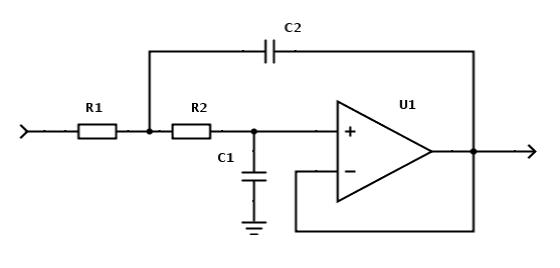
\includegraphics[width=1\textwidth]{Figurer/Hardware/FilterDesign}
	\caption{Unity gain 2. ordens Sallen-Key lavpas konfiguration}
	\label{fig:Filter}
\end{figure}

Et Butterworth-filter har en dæmpningsfaktor på 0,7, fordi der, i et Butterworth-filter, er blevet prioriteret et fladt frekvensområde, frem for hurtig dæmpning. Der blev brugt en hjemmeside som hjælpemiddel til at finde overføringsfunktionen for Butterworth-lavpasfilteret.\cite{Overforing} Denne ligning kan ses i ligning \ref{ligning5}:


\begin{align}
	\frac{V_{out}(S)}{V_{in}(S)}=\frac{\frac{1}{R_1C_1R_2C_2}}{s^2+s(\frac{1}{R_2C_2}+\frac{1}{R_1C_2})+\frac{1}{R_1C_1R_2C_2}}
	\label{ligning5}
\end{align}

Da det er blevet opgivet, at $R1=R2$ kan overføringsfunktionen forkortes, som set på ligning \ref{ligning6}.

\begin{align}
\frac{V_{out}(s)}{V_{in}(s)}=\frac{\frac{1}{R^2C_{1}C_{2}}}{s^2+s(\frac{2}{RC_{2}})+\frac{1}{R^2C_{1}C_{2}}}
\label{ligning6}
\end{align}

Dernæst sammenlignes med standardformlen for overføringsfunktionen for et andet ordens filter på figur \ref{ligning7}:

\begin{align}
\frac{V_{out}(s)}{V_{in}(s)} = \frac{\frac{1}{R^{2}C_{1} C_{2}}}{s^2+s(\frac{2}{RC_{2}})+\frac{1}{R^{2}C_{1}C_{2}}} = \frac{\omega_{0}^{2}}{s{2}+s(2\zeta\omega_{0})+\omega_{0}^{2}}
\label{ligning7}
\end{align}

Ud fra dette kan komponentværdierne regnes for R, idet vi har en opgivet værdi for $\frac{2}{RC_{2}}$, som vist på figur \ref{ligning8}:

\begin{align}
\frac{2}{RC_{2}}=2\zeta\omega_{0}
\label{ligning8}
\end{align}

Der blev herefter brugt Mathcad til at isolere R, og udregne værdien af denne. Dette kan ses på figur \ref{ligning9}:

\begin{align}
\frac{2}{R\cdot680\cdot10^{-9}}=2\cdot0.7\cdot(50\cdot2\cdot\pi) solve, R \to \frac{250000}{17\cdot\pi}=6.687\times 10^3
\label{ligning9}
\end{align}

Dernæst kan komponentværdien for C1 udregnes:


\begin{align*}
\frac{1}{R^2C_{1}C_{2}}=\omega_{0}^2
\label{ligning10}
\end{align*}	

Ved hjælp af Mathcad isoleres C1. 

\begin{align}
	\frac{1}{(6.687\times 10^{3})^{2}\cdot(680\cdot10^{-9})\cdot C_1}=(50\cdot 2\pi)^{2} solve, R \to 333,2\times 10^{-9}
\end{align}

Derved er komponentværdierne for kredsløbet fundet og kan ses indskrevet på \ref{fig:Filter}. 

\begin{figure}[H]
	\centering
	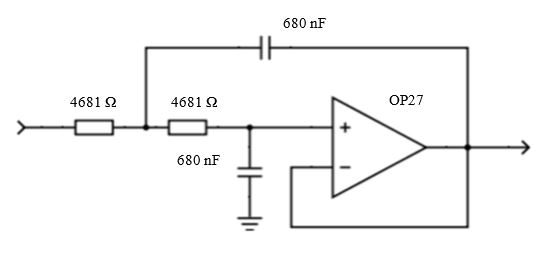
\includegraphics[width=1\textwidth]{Figurer/Hardware/FilterDesignMedKomponentvaerdier}
	\caption{Unity gain 2. ordens Sallen-Key lavpas konfiguration med indsatte komponentværdier.}
	\label{fig:Filter_K}
\end{figure}

For at underbygge teorien omkring filteret, blev der ved hjælp af værktøjet ”Sallen-Key Low-pass Filter Design Tool” udarbejdet et bodeplot \cite{Overforing}. Dette kan ses nedefor på figur \ref{fig:Bodeplot}. 

\begin{figure}[H]
	\centering
	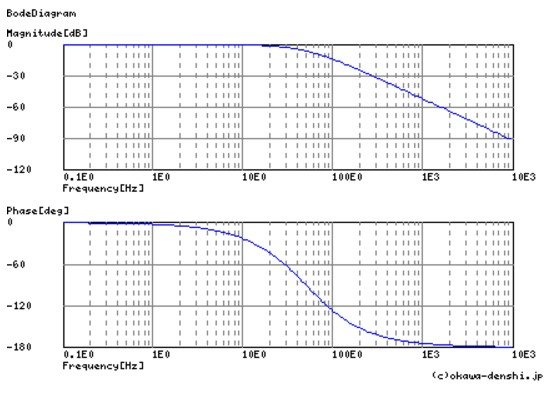
\includegraphics[width=1\textwidth]{Figurer/Hardware/Bodeplot}
	\caption{Bodeplot af overføringsfunktionen}
	\label{fig:Bodeplot}
\end{figure}



\subsection{Grænseflader}
Grænsefladerne for hardwareblokkene er beskrevet i tabel \ref{graenseflader}:

\begin{table}[H]
\centering
\small
\begin{tabular}{|l|l|l|l|l|}
\hline
\textbf{Navn} & \textbf{Input}  & \textbf{Output} & \textbf{Interval}                                                                   & \textbf{Beskrivelse}                                                                                                                                                                          \\ \hline
Transducer    & Tryk            & Spænding        & \begin{tabular}[c]{@{}l@{}}Ind; -50 mmHg\\ \\ Ud; 0 til 6,25 mV\end{tabular}        & \begin{tabular}[c]{@{}l@{}}Transduceren, i form af en \\ straingauge, reagerer i forhold\\  til trykændringer, og udsender\\  en spænding, som ændrer sig \\ i forhold til tryk.\end{tabular} \\ \hline
Forstærker    & Spænding        & Spænding        & \begin{tabular}[c]{@{}l@{}}Ind; 0 til 6,25 mV\\ \\ Ud; -2,5V til 2,5V\end{tabular}  & \begin{tabular}[c]{@{}l@{}}Forstærkeren modtager det svage\\  signal fra transduceren, og \\ forstærker signalet op, så det\\ matcher DAQ’ens dynamikområde.\end{tabular}                     \\ \hline
Filter        & Spænding        & Analogt signal  & \begin{tabular}[c]{@{}l@{}}Ind; -2,5V til 2,5V\\ \\ Ud; -2,5V til 2,5V\end{tabular} & \begin{tabular}[c]{@{}l@{}}Filteret modtager det forstærkede\\  signal fra forstærkeren og \\ filtrerer signalet.\end{tabular}                                                               \\ \hline
DAQ           & Analogt signal  & Digitalt signal & \begin{tabular}[c]{@{}l@{}}Ind; -2,5V til 2,5V\\ \\ Ud; -2,5V til 2,5V\end{tabular} & \begin{tabular}[c]{@{}l@{}}DAQ’en konverterer det analoge\\  signal fra filteret til et \\ digitalt signal, som computeren\\  modtager\end{tabular}                                       \\ \hline
Computer      & Digitalt signal & Grafisk billede &                                                                                     & \begin{tabular}[c]{@{}l@{}}Computeren modtager et digitalt\\  signal fra DAQ’en, som bliver \\ behandlet i koden.\end{tabular}                                                                \\ \hline
\end{tabular}
\caption{Grænsefladetabel}
\label{graenseflader}
\end{table}

\section{Software arkitektur}
\subsection{GUI}\label{GUI}
Dette afsnit beskriver, hvilke tanker og overvejelser der er gjort i forbindelse med designet af diverse brugergrænseflader. Nedenfor ses udkast til disse brugergrænseflader. Den endelige udgave af brugergrænseflader kan ses i afsnit \ref{implementering}.\\
Designet af brugergrænsefladen er blevet udført ud fra de 16 principper for gode brugergrænseflader \cite{Usability}. Der er ligeledes i "Form1"\ hentet inspiration fra allerede eksisterende blodtryksmonitor. I designet af brugergrænsefladen bestræbes der efter at gøre det så virkelighedsnært som muligt ud fra de redskaber og oplysninger, der er til rådighed.\\ \\
Brugergrænsefladen er inddelt i tre forskellige vinduer. De tre vinduer er henholdvis "Log ind"\,, "Form1"\ og "Gem"\.. De personer, der interagerer med brugergrænsefladen er sundhedsfagligt personale som typisk vil være en læge eller sygeplejerske. Dette er der også taget højde for i designet, da der aldrig vil være andre end det sundhedsfaglige personale, altså en skærpet målgruppe, der interagerer med brugergrænsefladen.\\
Nedenfor kommer der en uddybende beskrivelse af brugergrænsefladen. 

\begin{figure}[H]
	\centering
	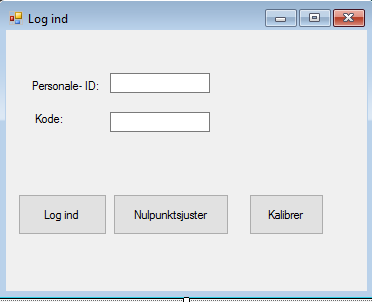
\includegraphics[width=0.7\textwidth]{Figurer/GUI/Logind_GUI}
	\caption{Login vindue}
	\label{Login vindue}
\end{figure}

I figur \ref{Login vindue} er der taget udgangspunkt i, at brugergrænsefladen skal være enkel og overskuelig opbygget. Der skal ikke være nogle overflødige ting og de knapper, der er vigtige som bruger skal benytte, skal stå tydeligt frem. Opbygningen skal afspejle brugerens logik.\\ \\ 
Tankerne omkring den enkle opbygning er, at hvis der opstår en akut situation, hvor systemet skal i gang hurtigt, skal det være nemt og hurtigt at logge ind i systemet. Det er vigtigt, at knapperne er selvforklarende og giver brugeren det, der forventes af knappen, når den benyttes. \\ \\
Der er taget højde for feedback til bruger. Ved forkert login får brugeren en besked om, at login er indtastet forkert, og der skal prøves forfra. \\


\begin{figure}[H]
	\centering
	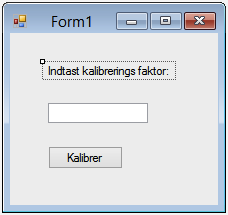
\includegraphics[width=0.5\textwidth]{Figurer/GUI/kalibrerGUI}
	\caption{Kalibrer vindue}
	\label{Kaliber vindue}
\end{figure}

Vist på figur \ref{Kaliber vindue}, hvor der her er lagt vægt på det funktionelle med et enkelt og simpelt design. Der er vejledende tekst, som gør det nemt for aktøren at finde ud af systemet.

\begin{figure}[H]
	\centering
	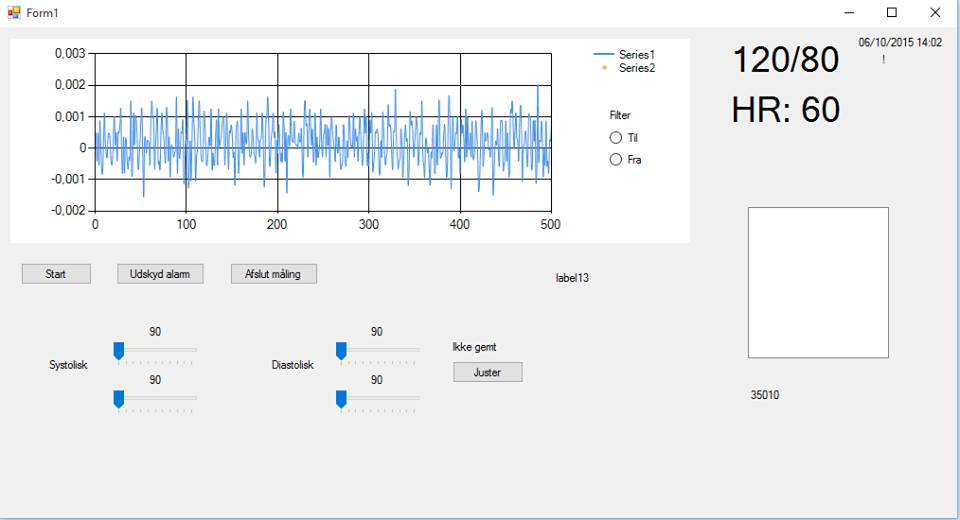
\includegraphics[width=1\textwidth]{Figurer/GUI/GUI_form1}
	\caption{Blodtryksvindue}
	\label{Blodtryk vindue}
\end{figure}

I blodtryksvinduet, vist på figur \ref{Blodtryk vindue}, er opbygningen mere kompliceret og med flere knapper end ved "Login"\ og "Gem”\.. Der er taget højde for, at knapperne er selvforklarende og deres navne afspejler de bagvedliggende handlinger. Dette medfører, at brugeren stadig har et overblik over brugergrænsefalden og stadig selv kan kontrollere hvad der skal ske. Denne brugergrænseflade er ikke tiltænkt nye brugere, men derimod brugere, der har et kendskab til den og til hvilke sundhedfaglige værdier og udtryk, der vises i vinduet.  Derfor benyttes brugerens sprog på brugergrænsefalden, altså med fagtermer. 

\begin{figure}[H]
	\centering
	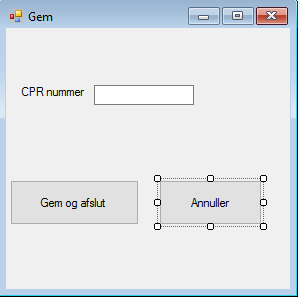
\includegraphics[width=0.7\textwidth]{Figurer/GUI/Gem_GUI}
	\caption{"Gem"\ -vindue}
	\label{Gem vindue}
\end{figure}

På figur \ref{Gem vindue}, "Gem"\--vinduet, er der igen taget udgangspunkt i en enkel opbygning og at knapperne, der skal bruges er tydelige og selvforklarende. Det er her også brugerens logik, der afspejles og ingen unødvendige ting er inddraget i brugergrænsefladen. Det er her muligt at afbryde situationen ved, at der er en alternativ udvej, som kan bruges, hvis den opstartede handling fortrydes. Der er taget højde for feedback til brugeren, hvis der indtastes forkert CPR-nummer, får brugeren det at vide i et pop op-vindue. 

\subsection{Domænemodel}
Diagrammet viser en domænemodel for blodtryksmålingssystemet. Dette diagram giver et godt overblik over systemet som helhed og hvilke elementer, der indgår i systemet. Diagrammet viser, hvordan brugeren interagerer med systemet, og hvordan systemet forløber, efter det igangsættes af bruger. 

\begin{figure}[H]
	\centering
	\includegraphics[width=1\textwidth]{Figurer/ISE/Domaenemodel}
	\caption{Domænemodel}
	\label{domaenemodel}
\end{figure}

\subsection{Appliktationsmodel}
Applikationsmodellen er en model der på baggrund af domænemodel og use cases udarbejdes software-relaterede klasse-applikationsmodeller, sekvensdiagrammer og opdaterede klasse-applikationsmodeller.\\
Her er det ikke-opdateret klassediagram udeladt, hvorfor sekvensdiagram og opdaterede klasse-applikationsmodel er udarbejdet på baggrund af fiktive metoder. De faktiske metoder kan ses i afsnit \ref{UML klassediagram}.

\subsubsection{Sekvensdiagram}
Sekvensdiagrammet er et interaktionsdiagram, der viser, hvordan processer i systemet forløber. Use casene ligger til baggrund for udarbejdelsen af sekvensdiagrammerne.\\ \\
Der er blevet lavet et sekvensdiagram for hver use case for at give det bedste overblik over hver handling i forhold til systemet. I sekvensdiagrammet har vi brugt virtuelle metodekald til at beskrive forløbet. I use case 2-7 er det brugeren, der interagerer med systemet og er initiator for, at handlingerne bliver udført.

\begin{figure}[H]
	\centering
	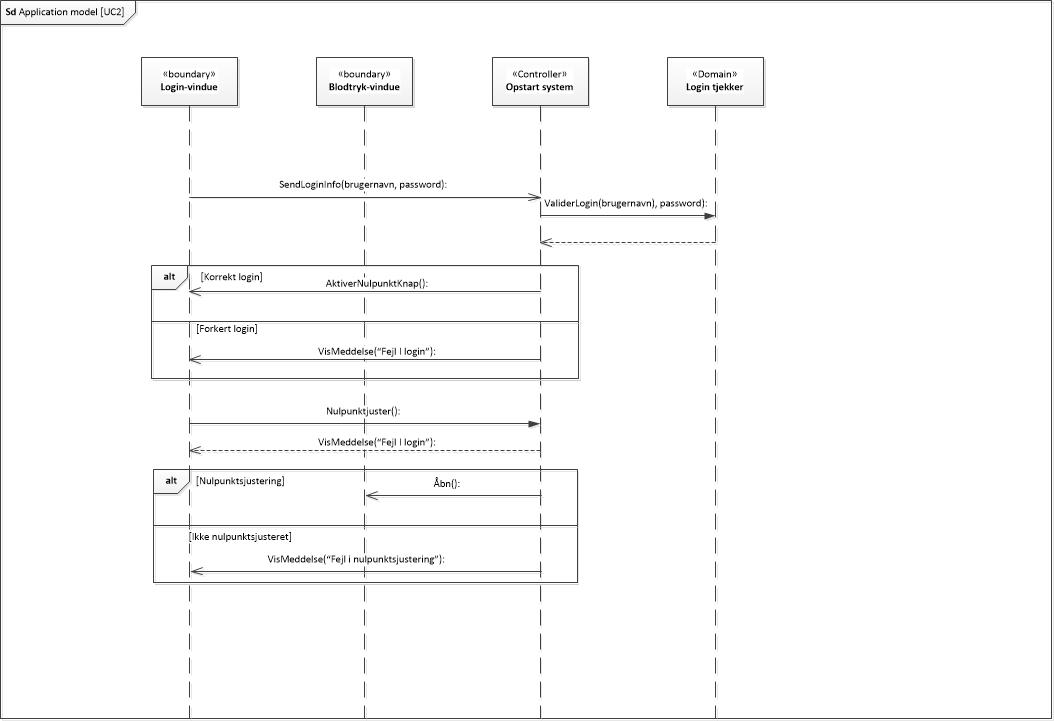
\includegraphics[width=1\textwidth]{Figurer/ISE/sdAppModelUC2}
	\caption{Sekvensdiagram UC2}
	\label{sd UC2}
\end{figure}

På figur \ref{sd UC2} ses det, hvordan brugeren logger ind i systemet, og hvordan brugeren får systemet nulpunktsjusteret. Det er brugeren, der interagerer med systemet og er initiator for, at handlingerne bliver udført. 

\begin{figure}[H]
	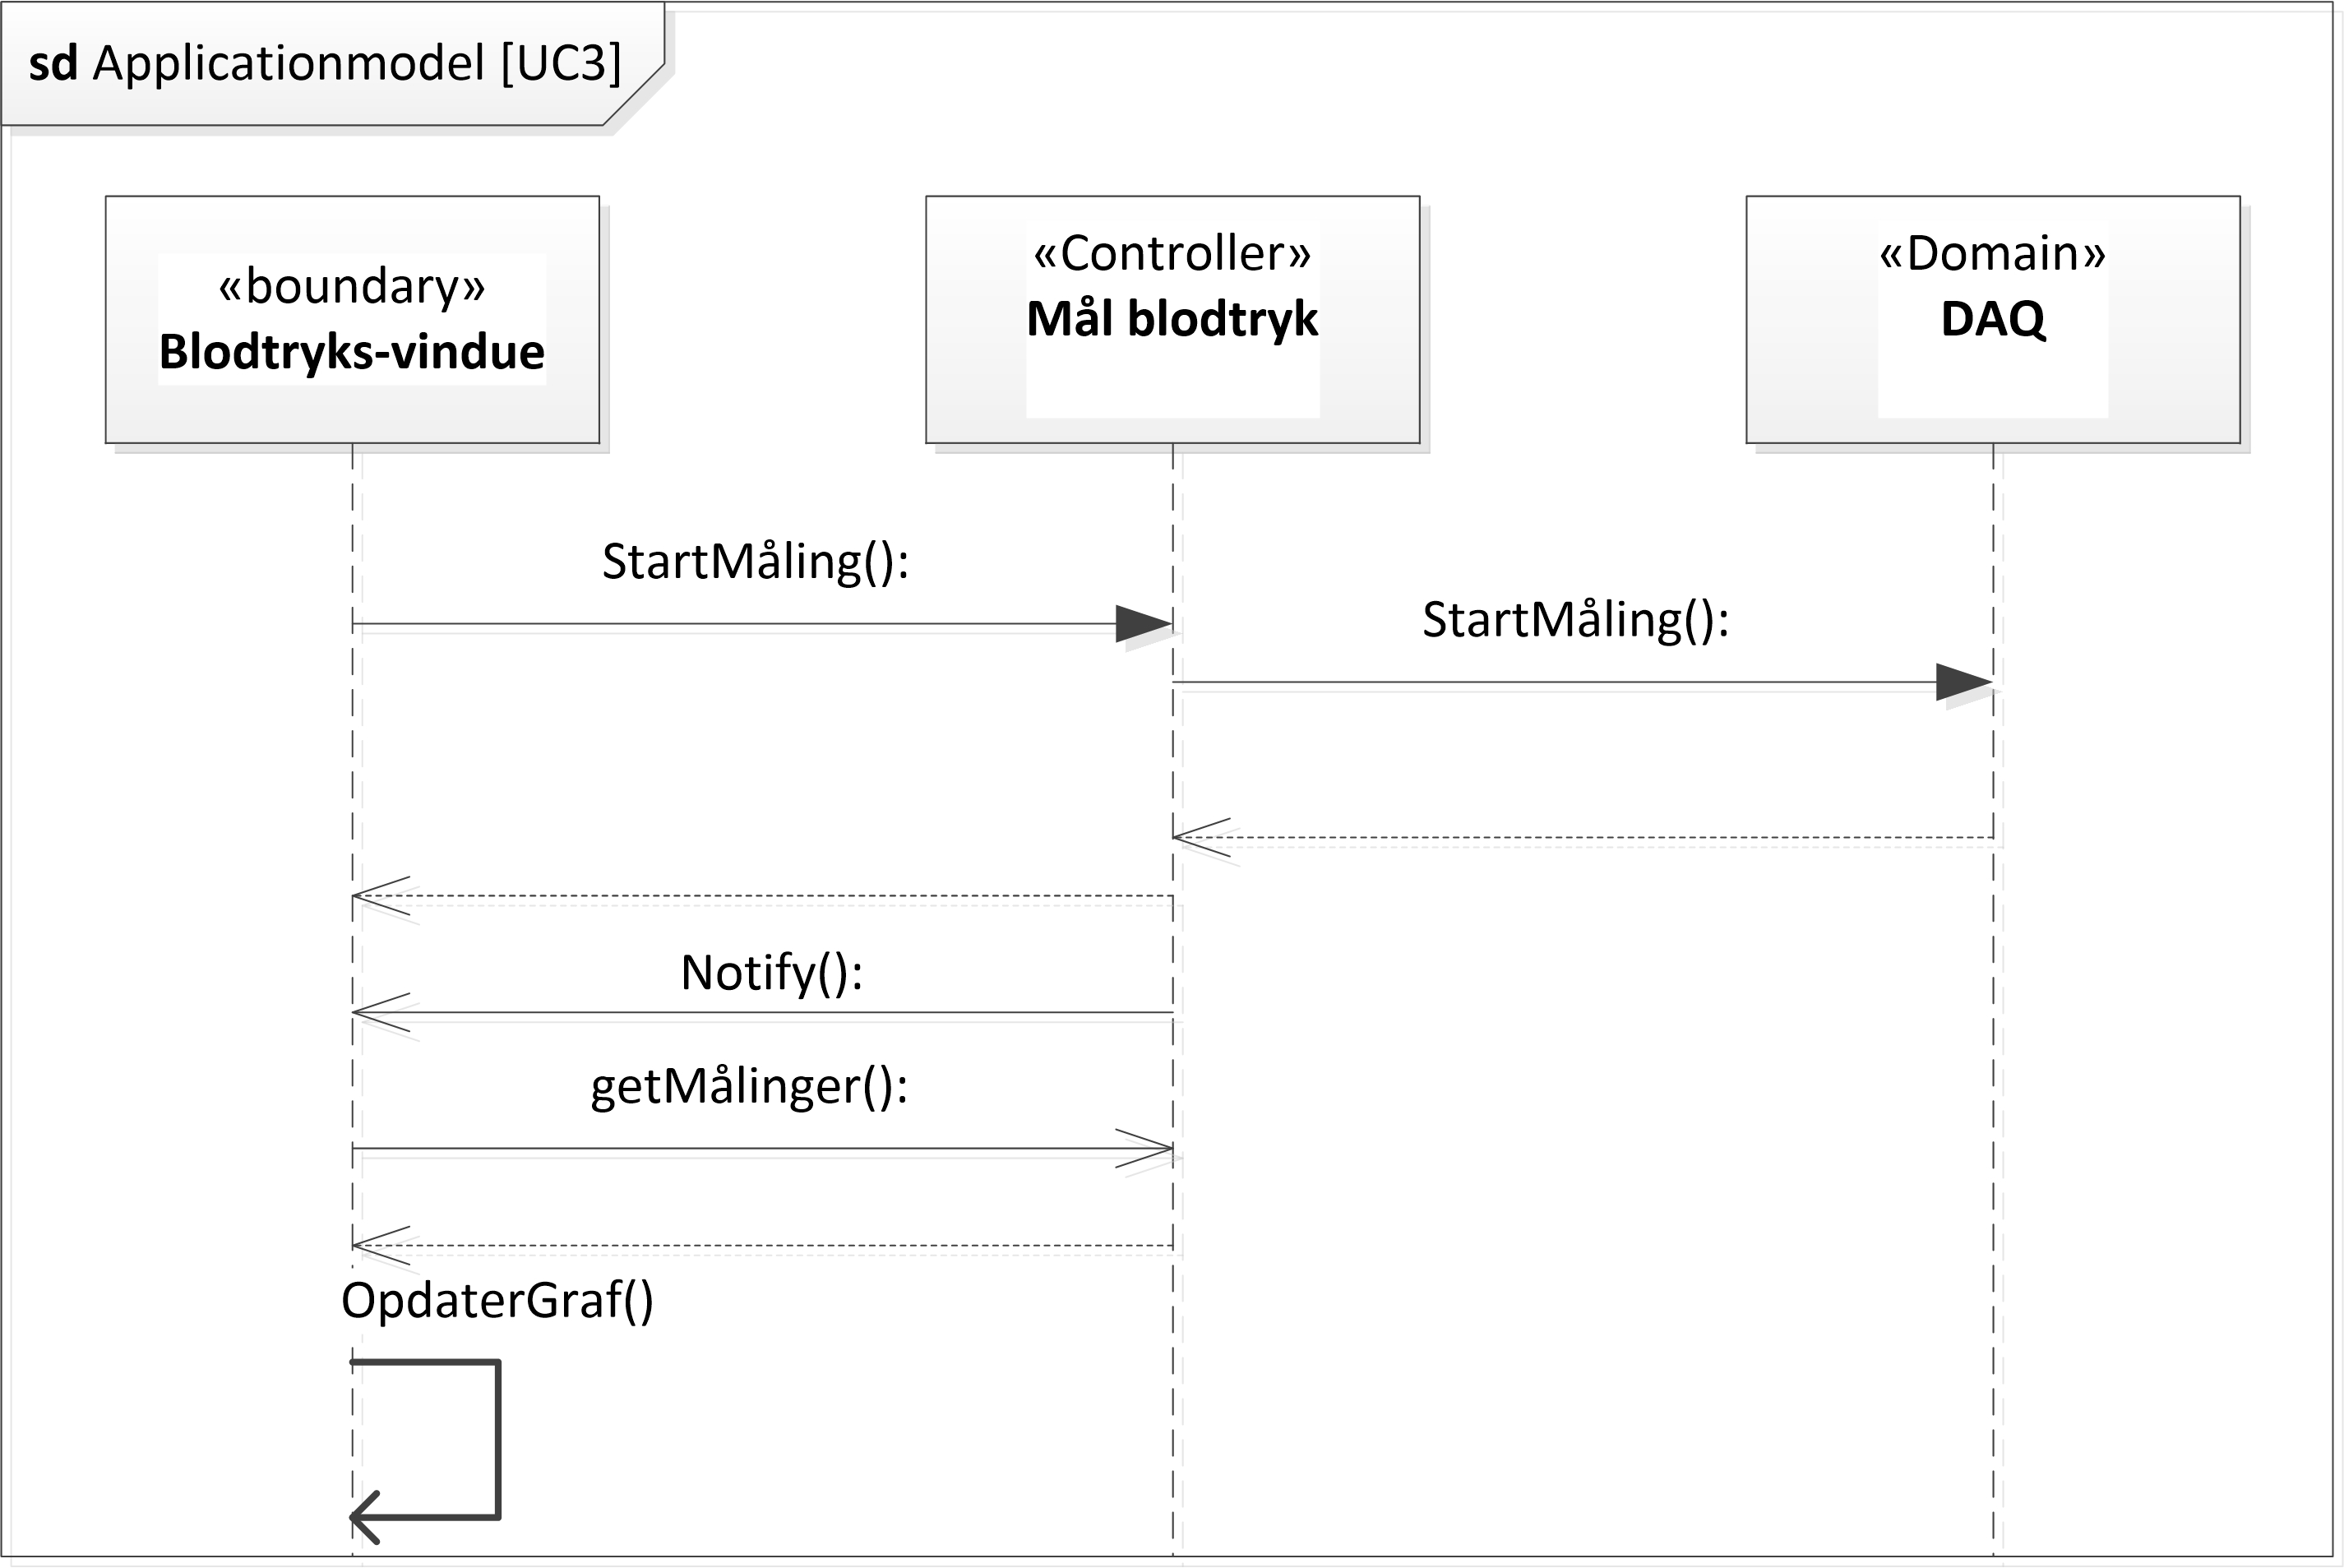
\includegraphics[width=1\textwidth]{Figurer/ISE/sdAppModelUC3}
	\caption{Sekvensdiagram UC3}
	\label{sd UC3}
\end{figure}

Figur \ref{sd UC3} viser, hvordan brugeren starter målingen, og hvordan graferne vises på brugergrænsefladen.

\begin{figure}[H]
	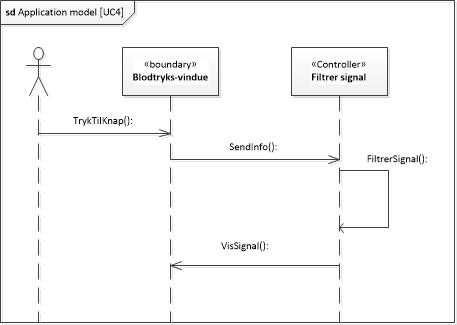
\includegraphics[width=0.7\textwidth]{Figurer/ISE/sdAppModelUC4}
	\caption{Sekvensdiagram UC4}
	\label{sd UC4}
\end{figure}

I sekvensdiagrammet figur \ref{sd UC4} ses, hvordan brugeren kan vælge om blodtrykssignalet skal filtreres eller ej.

\begin{figure}[H]
	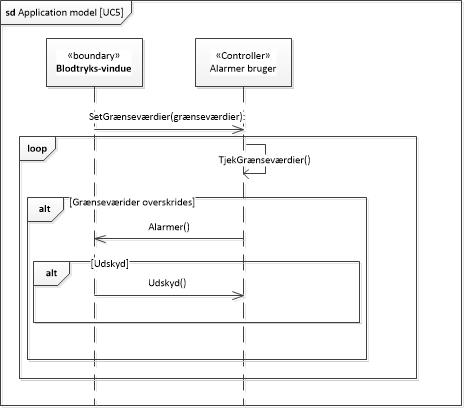
\includegraphics[width=1\textwidth]{Figurer/ISE/sdAppModelUC5}
	\caption{Sekvensdiagram UC5}
	\label{sd UC5}
\end{figure}

Det ses på figur \ref{sd UC5}, hvordan brugeren justerer grænseværdierne for patientens blodtryk. Denne justering sker ud fra patientens målte blodtryk. De justerede grænseværdier ligger til grundlag for alarmen. Desuden viser figuren, at brugeren har mulighed for at udskyde alarmen.

\begin{figure}[H]
	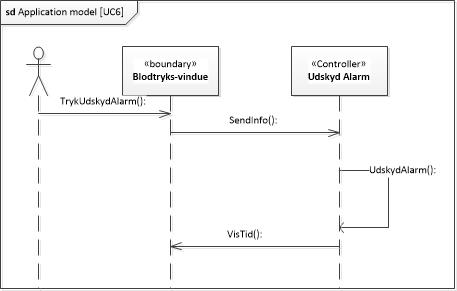
\includegraphics[width=1\textwidth]{Figurer/ISE/sdAppModelUC6}
	\caption{Sekvensdiagram UC6}
	\label{sd UC6}
\end{figure}

Figur \ref{sd UC6} viser, hvordan systemet gemmer og afslutter en måling. 

\subsubsection{Opdateret applikationsmodel}
Klasse-applikationsmodellerne er udarbejdet ud fra use casene, sekvensdiagrammer og domænemodellen. Der er ligesom ved sekvensdiagrammerne lavet et klassediagram for hver use case. Der er også her brugt virtuelle metoder. 

\begin{figure}[H]
	\centering
	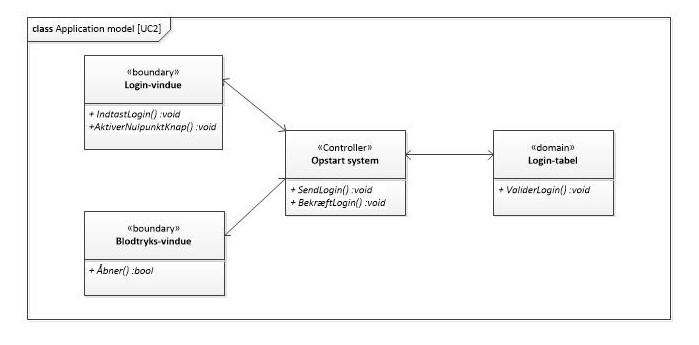
\includegraphics[width=1\textwidth]{Figurer/ISE/classAppModelUC2}
	\caption{Klassediagram UC 2}
	\label{classApp UC2}
\end{figure}

\begin{figure}[H]
	\centering
	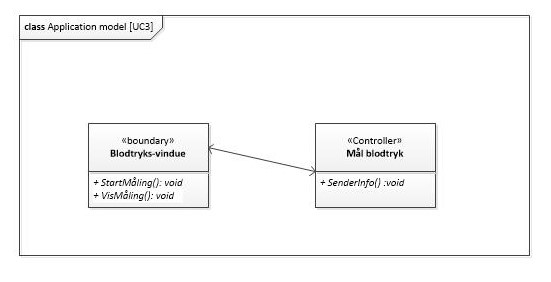
\includegraphics[width=1\textwidth]{Figurer/ISE/classAppModelUC3}
	\caption{Klassediagram UC 3}
	\label{classApp UC3}
\end{figure}

\begin{figure}[H]
	\centering
	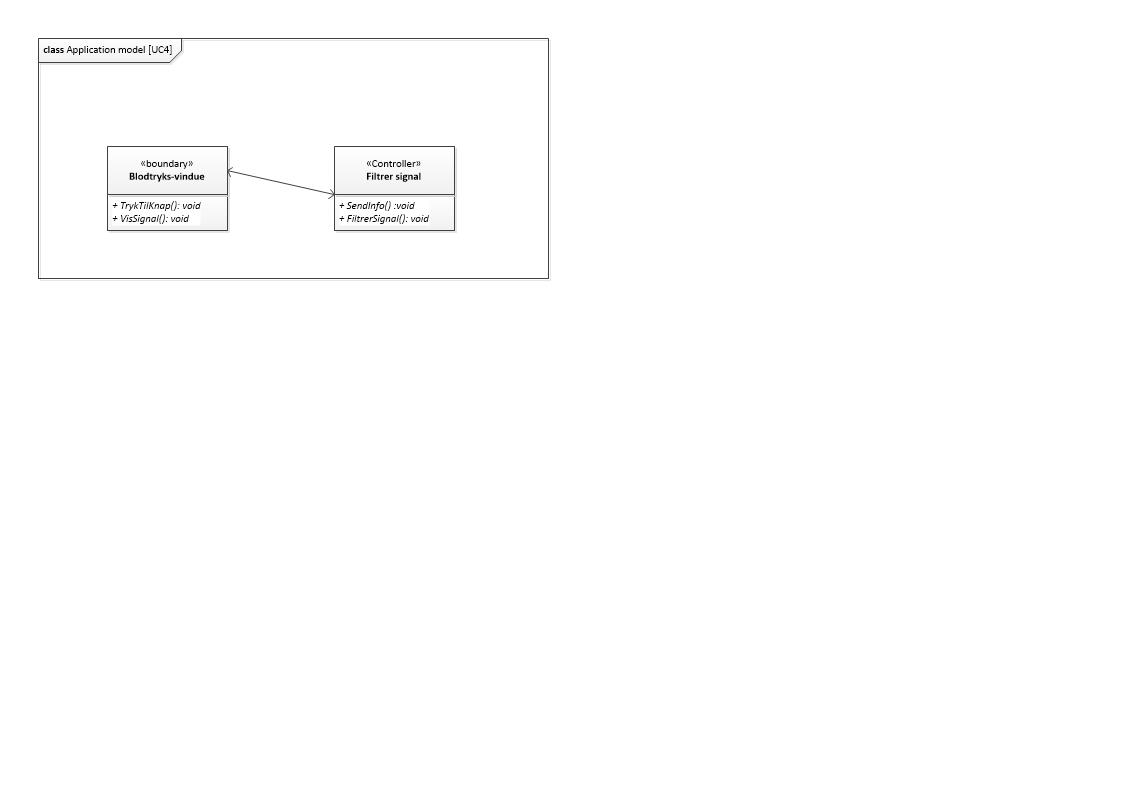
\includegraphics[width=1\textwidth]{Figurer/ISE/classAppModelUC4}
	\caption{Klassediagram UC 4}
	\label{classApp UC4}
\end{figure}

\begin{figure}[H]
	\centering
	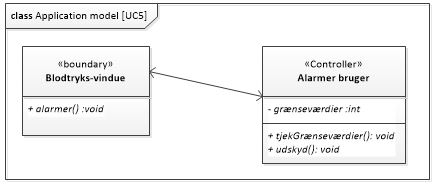
\includegraphics[width=1\textwidth]{Figurer/ISE/classAppModelUC5}
	\caption{Klassediagram UC 5}
	\label{classApp UC5}
\end{figure}

\begin{figure}[H]
	\centering
	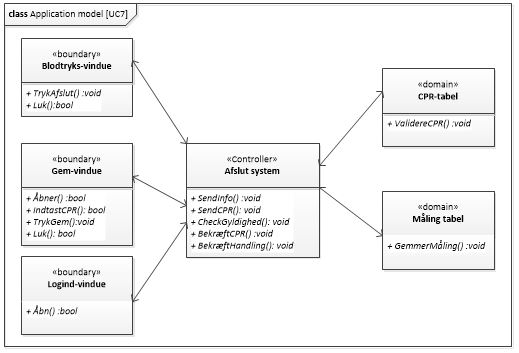
\includegraphics[width=1\textwidth]{Figurer/ISE/classAppModelUC7}
	\caption{Klassediagram UC 7}
	\label{classApp UC7}
\end{figure}

\chapter{Implementering}\label{Implementering}

\begin{longtabu} to \linewidth{@{}l l l X[j]@{}}
    Version &    Dato &    Ansvarlig &    Beskrivelse\\[-1ex]
    \midrule
    0.1 &	8/09 2015	&	Alle		& Oprettelse  af dokument\\
    0.2 &	07/12 2015 	& SSK, NHL, FRM & Påbegyndelse af hardware implementeringsafsnit\\
    0.3 &	10/12 2015 	& TSN, JTH, MFJ & Påbegyndelse af software implementeringsafsnit \\
\label{version implementering}
\end{longtabu}

\section{Hardware implementering}\label{Hardware implementering}

Efter teorifasen blev de to blokke bygget op. Forstærkeren og filteret blev bygget på hver sit fumlebræt, dels på grund af pladsmangel og dels på grund af større sammenhæng mellem arkitekturen og det endelige produkt.\\

\begin{figure}[H]
	\centering
	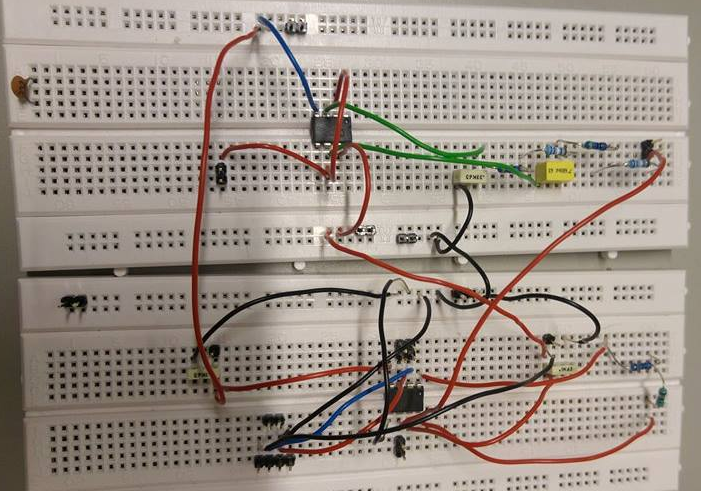
\includegraphics[width=1\textwidth]{Figurer/Hardware/samletopstilling}
	\caption{Opstilling af forstærker og filter}
	\label{Dsamletopbygning}
\end{figure}

\subsubsection{Hardware overvejelser}

I udviklingen af hardwaren, opstod der problemstillinger, som  gjorde, at der var nogle komponentvalg, som var nødvendige at genoverveje.\\
\\
Et af de største problemer var brugen af  operationsforstærker i forstærkerblokken. En reel operationsforstærker har ikke en uendelig indgangsmodstand, som i den ideelle verden, og der er derfor en risiko for, at den lave spænding fra transduceren simpelthen ikke ville kunne passere forstærkeren. Det blev derfor valgt at bruge en instrumentationsforstærker i stedet, da den reelle komponents egenskaber ligger langt tættere på dens ideelle modpart, og derfor var bedre egnet i kredsløbet. En anden fordel ved instrumentationsforstærkeren er, at den er meget let at justere forstærkning på.\\
\\
En anden stor fordel ved instrumentationsforstærkeren er, at common mode rejection ratio er meget høj. Common mode noise er støj, fra det omkringliggende miljø. Da en instrumentationsforstærkers forstærkning kommer fra forskellen mellem dens to indgange, kan støj påvirke forstærkningen, især når der arbejdes med så lave forstærkninger, som dem, der kommer fra transduceren. Ofte er der dog støj på begge indgange, og i den ideelle verden ville dette ikke påvirke forstærkningen. I den reelle verden kan støjen dog også ende med at blive forstærket. Common mode rejection ratio beskriver hvor god en komponent er til at sortere støj fra. Den brugte instrumentationsforstærker har en common mode rejection ratio på 120 dB, hvilket vurderes til en fornuftig værdi. \\
\\
En anden ting ved forstærkeren, som blev nødt til at blive ændret, var det dynamik område, som skulle udnyttes. Oprindeligt havde gruppen bestemt, at det filtrerede signal skulle ligge imellem -5V og +5V. Grundet en forstærkers manglende evne til at forstærke et signal op til dens forsyningsspænding, så blev det vurderet, at det var nødvendigt at nedsætte signalområdet fra -2,5V til +2,5V. Det var muligt at forstærke signalet yderligere, men grænsen blev sat til denne værdi, fordi signalområdet matcher et dynamikområde på DAQ'en.\\ 
\\
Designet af filteret, lå fast på forhånd, og der var derfor ikke meget der kunne ændres i dette. Operationsforstærkeren var oplyst til at skulle være af typen OP27, da denne ligeledes har en god common mode rejection. Grundet mangel på præcise komponenter, blev der sat to modstande i serie, for at komme så tæt på den udregnede værdi, som muligt. \\
\\
Det blev desuden valgt at systemet skulle forsynes af Analog Discovery, frem for et batteri. Dette skyldes at Analog Discovery giver en stabil strøm, som ikke har brug for at blive afbalanceret af en spændingsudligner. Det blev vurderet at usikkerhederne ville udligne hinanden, og der var flere fordele ved at bruge Analog Discovery.\\


\subsubsection{Implementering af forstærkeren}
Den samlede stykliste for forstærkeren er vist i tabel \ref{DForsttabel}:

\begin{table}[H]
\centering
\begin{tabular}{|l|l|l|ll}
\cline{1-3}
\textbf{Komponent} & \textbf{Antal} & \textbf{Type}  &  &  \\ \cline{1-3}
Modstand           & 1              & 120 $\Omega$   &  &  \\ \cline{1-3}
Modstand           & 1              & 4.8 $\Omega$   &  &  \\ \cline{1-3}
Kondensator        & 2              & 100 nF         &  &  \\ \cline{1-3}
Instrumentationsforstærker &    1   & INA114		     &  &  \\ \cline{1-3}
\end{tabular}
\caption{Forstærkertabel}
\label{DForsttabel}
\end{table}

For forstærkeren gælder det, at den beregnede R$_{gain}$ er 125,31$\Omega$ som det kan ses ud af komponentlisten består R$_{gain}$ i praksis af to modstande på henholdsvis 4,8$\Omega$ og 120$\Omega$, som er sat i serie. R$_{gain}$ modstanden er i praksis 124,8$\Omega$. I praksis er R$_{gain}$ 0,51$\Omega$ mindre end den i teorien skulle have været.

\subsubsection{Implementering af filteret}
Den samlede stykliste for filteret er som vist på tabel \ref{DFiltertabel}:

\begin{table}[H]
\centering
\begin{tabular}{|l|l|l|ll}
\cline{1-3}
\textbf{Komponent} & \textbf{Antal} & \textbf{Type}  &  &  \\ \cline{1-3}
Modstand           & 2              & 6.2 k $\Omega$ &  &  \\ \cline{1-3}
Modstand           & 2              & 470 $\Omega$   &  &  \\ \cline{1-3}
Kondensator        & 1              & 680 nF         &  &  \\ \cline{1-3}
Kondensator        & 1              & 330 nF         &  &  \\ \cline{1-3}
Operationsforstærker &    1         & OP27G          &  &  \\ \cline{1-3}
\end{tabular}
\caption{Filtertabel}
\label{DFiltertabel}
\end{table}

Det analoge filter består blandt andet af en 330 nF kondensator, C$_1$, som i teorien er beregnet til at skulle have været 333,2 nF. I praksis er kondensatoren C$_1$ 3,2 nF mindre, end den i teorien er beregnet til at skulle have været. Filteret består desuden af to modstande R$_1$ og R$_2$, som er identiske. I det realiserede analoge filter består hver modstand af to modstande på henholdsvis 6200$\Omega$ og 470$\Omega$, som er sat i serieforbindelse. Dermed er både R$_1$ og R$_2$ 6670$\Omega$ i praksis. I teorien var R$_1$ og R$_2$ udregnet til at skulle være 6687$\Omega$. I praksis er modstanden derfor 17$\Omega$ mindre end teorien foreskriver.\\

Generelt er der valgt at se bort fra de afvigelser, der er for komponentværdierne i praksis sammenlignet med de i teorien beregnet. Det er valgt da afvigelserne er relativt små i forhold til det pågældende komponent. For modstandende er der desuden 1\% usikkerhed, hvilket betyder, at man alligevel ikke kan være helt sikker på komponentværdien.\\

På baggrund af de i praksis anvendte komponenter er den reelle knækfrekvens for det analoge filter beregnet. Til det formål er formlen som set på figur \ref{dcutoff]} anvendt.\\

\begin{align}
f_{c} = \frac{1}{2\pi \sqrt{R_{1}C_{1}R_{2}C_{2}}} = \frac{1}{2\pi \sqrt{6687 \cdot 333,2\times 10^{-9} \cdot 6687 \cdot 680\times 10^{-9}}} = 50,37 Hz
	\label{dcutoff}
\end{align}

Desuden er den reelle $\zeta$ for dette filter, ifølge Okawa-Denshi, 0,697.


\section{Software implementering}\label{implementering}
Implementeringsafsnittet beskriver, hvilke faktiske handlinger der er foretaget ud fra arkitektur- og designafsnittet. Yderligere beskriver afsnittet, hvilke softwareorienterede metoder, der er benyttet, for at løse problemstillingen.

\subsection{3-lagsmodellen}
Softwaren er først og fremmest implementeret ud fra 3-lagsmodellen.\\
3-lagsmodellen er bestående af lagene præsentationslag, logiklag og datalag.
Denne opdeling af lagene gør det langt lettere at vedligeholde systemet, fordi der kan ændres i et enkelt lag, uden det har indflydelse på resten af programmet. \\
3-lagsmodellen er desuden en god softwarearkitektur at bruge til  systemudarbejdelse, når der arbejdes i grupper. Dette skyldes, at der kan arbejdes på to forskellige lag af to personer samtidigt, hvis bare grænsefladerne bliver overholdt. 3-lagsmodellen er bygget op som vist på figur \ref{3lag}:

\begin{figure}[H]
	\centering
	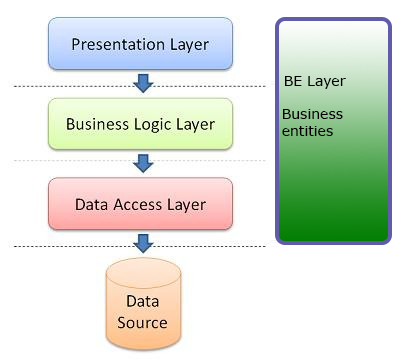
\includegraphics[width=0.8\textwidth]{Figurer/SoftwareImplementering/3lag}
	\caption{3-lagsmodellen}
	\label{3lag}
\end{figure}

\subsubsection{Præsentationslag}\label{praesentationslag}

Som vist på figur \ref{3lag}, er blodtrykssystemet bygget op med først et præsentationslag bestående af tre vinduer, som brugeren kan interagere med.\\
"Login"\--vinduet, bestående af tekstbokse til brugernavn og kodeord, samt paneler til både kalibrering og nulpunktsjusteringen, som vist på figur \ref{LoginGUI}:

\begin{figure}[H]
	\centering
	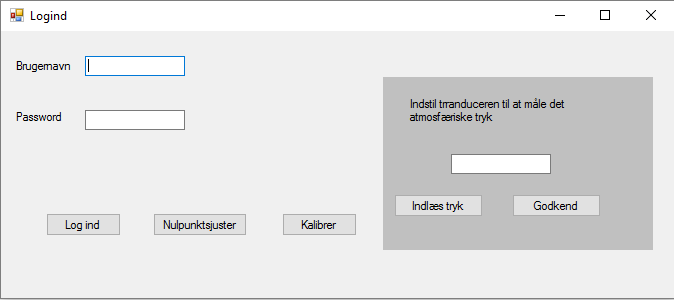
\includegraphics[width=1\textwidth]{Figurer/SoftwareImplementering/Logind}
	\caption{Login GUI}
	\label{LoginGUI}
\end{figure}
Dernæst åbnes hovedvinduet, hvor blodtrykssignalet vises grafisk, samt brugeren har mulighed for at benytte en række funktioner i form af knapper og trackbars, som set på figur \ref{form1}

\begin{figure}[H]
	\centering
	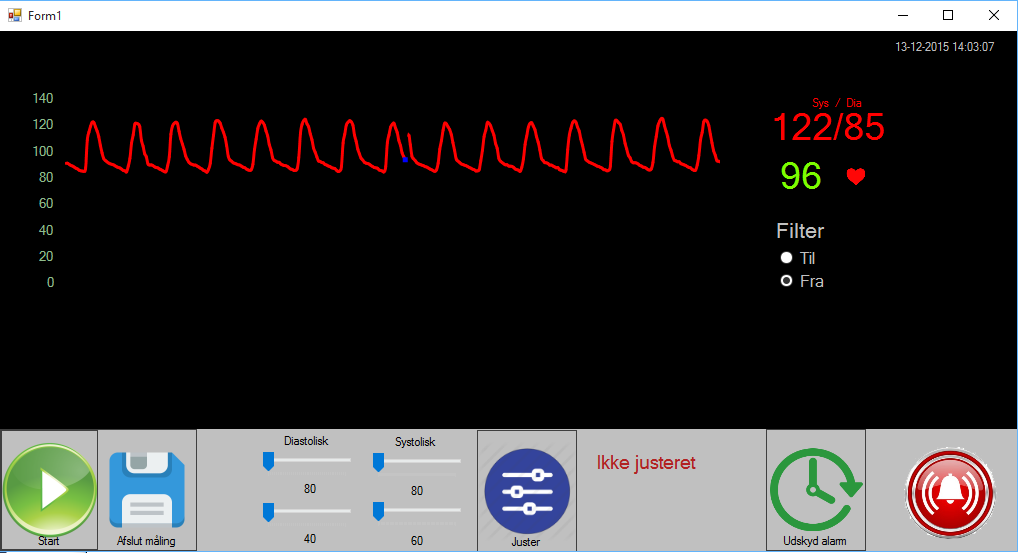
\includegraphics[width=1\textwidth]{Figurer/SoftwareImplementering/blodtryk}
	\caption{Blodtrykssystem hoved brugergrænseflade}
	\label{form1}
\end{figure}

Til sidst vises et vindue for gemmefunktionen, hvor brugeren skal indtaste et CPR-nummer, samt bekræfte afslutning af målingen, se figur \ref{Gem}:

\begin{figure}[H]
	\centering
	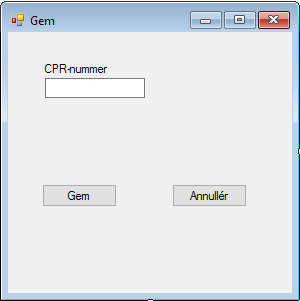
\includegraphics[width=0.6\textwidth]{Figurer/SoftwareImplementering/Gem}
	\caption{Gem GUI}
	\label{Gem}
\end{figure}

\subsubsection{Logiklag}\label{Logiklag}
Logiklaget er det lag, der spiller sammen med både data- og præsentationslag. Sammenspillet med præsentationslaget fungerer ved brugerens interaktion med systemet bearbejdes i logiklaget. Et eksempel herpå er det digitale filter, hvor brugeren gennem brugergrænsefladen tilslutter filteret. Dette igangsætter en metode i logiklaget, som sørger for, at signalet filtreres. Metoden er vist i figur \ref{filtrer} og figur \ref{Filtrer}:

\begin{figure}[H]
	\centering
	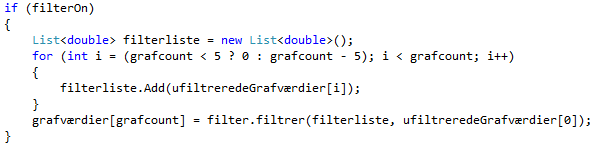
\includegraphics[width=1.15\textwidth]{Figurer/SoftwareImplementering/Filtrer1}
	\caption{Dataudvælgelse funktionen i logik-klassen}
	\label{Filtrer}
\end{figure}

\begin{figure}[H]
	\centering
	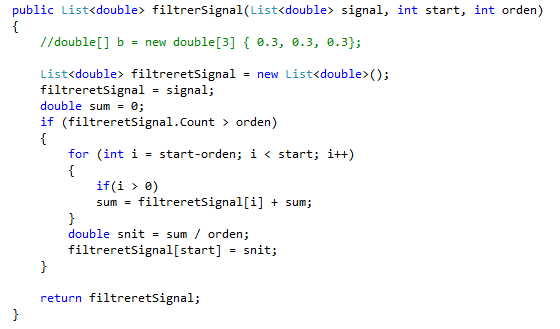
\includegraphics[width=0.85\textwidth]{Figurer/SoftwareImplementering/filtrer}
	\caption{Filtrer() i filter-klassen}
	\label{filtrer}
\end{figure}

Figur \ref{Filtrer} tager fem værdier og sender videre til filtrer(), som tager gennemsnittet på disse værdier, hvorefter gennemsnittet sendes tilbage til logik-klassen.
Dette kaldes for moving average, som er en form for FIR-filter.

\subsubsection{Datalag}\label{Datalag}
Datalaget er det lag, som spiller sammen med databasen og logiklaget. Det vil sige, at datalaget modtager brugerinputs fra brugergrænsefladen gennem logiklaget. Herefter henter datalaget informationer i en database, som efterfølgende sendes retur til logiklaget. Eksempelvis bliver login-oplysninger tjekket i databasen via datalaget, hvilket er vist i figur \ref{Datalogin}:

\begin{figure}[H]
	\centering
	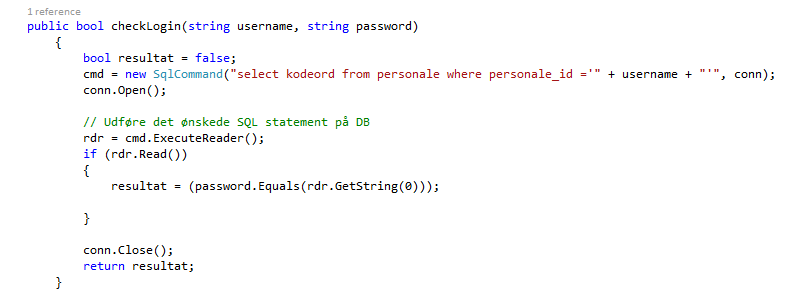
\includegraphics[width=1.4\textwidth]{Figurer/SoftwareImplementering/CheckLogind}
	\caption{checkLogin()}
	\label{Datalogin}
\end{figure}

Figur \ref{Datalogin} viser, hvordan checkLogin() opretter forbindelse til en privat database, hvorefter de indtastede værdier tjekkes i databasen. Til slut lukkes forbindelsen igen. Værdierne, der tjekkes med, kan ses i personale-tabellen i databasen, som vist i figur \ref{personaletabel}:

\begin{figure}[H]
	\centering
	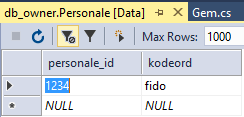
\includegraphics[width=0.6\textwidth]{Figurer/SoftwareImplementering/database}
	\caption{Personale-tabel}
	\label{personaletabel}
\end{figure}

Herudover er det også i datalaget, at data bliver indlæst fra DAQ'en. Dette gøres ved at udnytte, at DAQ'en har et asynkront kald i sig. Dette asynkrone kald gør, at der bliver leveret data fra DAQ til datalag løbende istedet for i intervaller, som ville være tilfældet ved synkrone kald. Det asynkrone kald tillader altså, at portioner af koden bliver udført løbende. 

\subsection{Tråde}
Blodtrykmålingssystemet skal simultant opfange målinger og vise disse på brugergrænsefladen. Dette stiller nogle krav til softwareopbygningen, da kodestykker skal køre på samme tid. For at løse denne problemstilling, er der anvendt trådprogrammering. Trådprogrammering er et integreret værktøj i C\#, som giver mulighed for at køre flere ting samtidigt på flere kerner i computerens CPU.\\
Softwaren er opbygget efter 3-lagsmodellen, og der findes en tråd i hvert lag, som har forskellige opgaver. \\
I datalaget laver DAQ-klassen asynkrone kald, når der skal opsamles målinger fra hardwareenheden. Ved at lave asynkrone kald vil opsamlingsprocessen køre i en tråd for sig selv, hvilket forhindrer at programmet låser, mens der måles. Et eksempel herpå ses på figur \ref{Traad}:

\begin{figure}[H]
	\centering
	\includegraphics[width=0.8\textwidth]{Figurer/SoftwareImplementering/Traad}
	\caption{Kodestykke fra startMåling() i klassen "DAQklasse". Her ses det, der er anvendt et asynkront kald}
	\label{Traad}
\end{figure}

I logiklaget er der også en tråd, og denne tråd sørger for at opsamle og behandle data fra datalaget. Ved at anvende en tråd her, er der mulighed for at udføre logiske operationer på datamængden, såsom filtrering, og sende denne videre til grafen i præsentationslaget.\\
Når man arbejder med Windows Forms i C\#, vil disse pr. automatik ligge i sin egen tråd, hvilket deraf også er tilfældet her.\\
For at opdatere form-elementer fra en anden tråd, skal disse opdateres gennem en invoke-metode. Dette betyder, at tråden tjekker, om den kan komme til, og hvis det er tilfældet, opdateres elementet, som vist i figur \ref{callback}:

\begin{figure}[H]
	\centering
	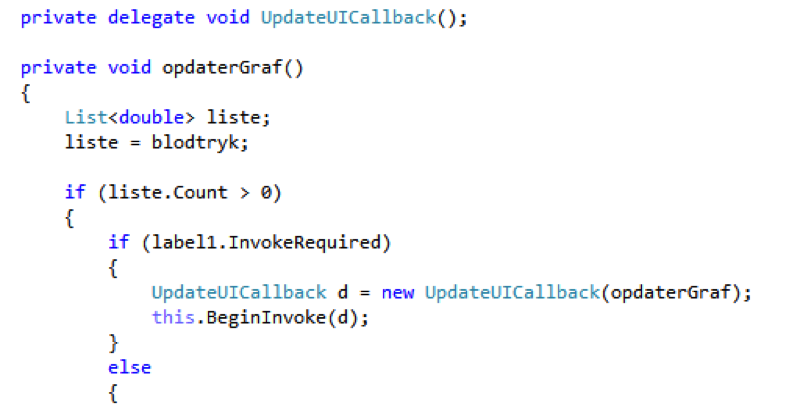
\includegraphics[width=0.9\textwidth]{Figurer/SoftwareImplementering/callback}
	\caption{Eksempel på en UpdateUICallback. Metoden kalder sig selv ind til den har fået udført kodestykkerne, der efterfølger "else"\ }
	\label{callback}
\end{figure}

Der er også andre ting, man skal være opmærksom på, når man arbejder med tråde. Der har i programmeringsarbejdet været problemer med, at der opstår en konflikt, når to tråde prøver at skrive til det samme objekt på samme tid.\\
For at imødekomme dette problem, er der anvendt en lås i form af en "mutex"\.. På denne måde forhindre man, at datalagets dataopsamler skriver til den samme liste, som logiklaget er i gang med at udføre logiske operationer på, vist på figur \ref{mutex}:

\begin{figure}[H]
	\centering
	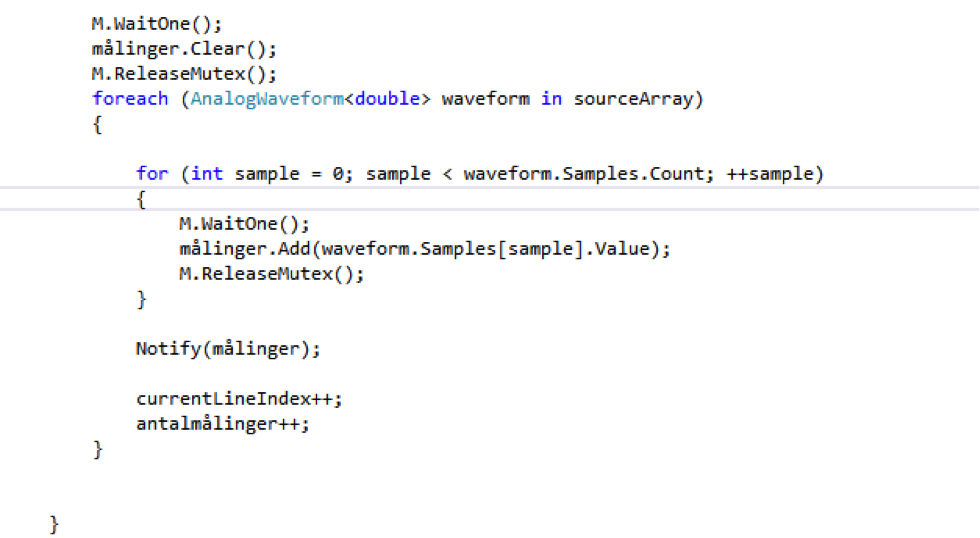
\includegraphics[width=1.1\textwidth]{Figurer/SoftwareImplementering/mutex}
	\caption{Eksempel på en UpdateUICallback. Metoden kalder sig selv ind til den har fået udført kodestykkerne, der efterfølger "else"\ }
	\label{mutex}
\end{figure}


\subsection{Observer-pattern}
Observermønstret er et mønster, hvor et objekt, kaldet et subject, informerer en liste af observers, når noget er ændret eller gennemført ved at kalde en af deres metoder. Dette mønster har været nødvendigt at anvende, da grafen i præsentationslaget skal informeres om, hvornår der er nye data af hhv. logiklaget og datalaget. Det vil sige, at Logik-klassen og DAQ-klassen begge fungerer som subjects, mens GUI-laget og Logik-klassen fungerer som observers. Logik-klassen er subject for GUI, og Data-klassen er subject for Logik.\\
Mønstret er sat op ved at lave to interfaces, ISubject og IObserver, som de respektive klasser arver fra og tvinges dermed til at implementere metoderne, som er beskrevet i interfaces. Dette ses i de tre efterfølgende figurer, figur \ref{observer1},\ref{observer2}, \ref{observer3}:

\begin{figure}[H]
	\centering
	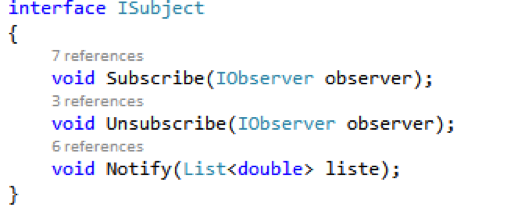
\includegraphics[width=0.6\textwidth]{Figurer/SoftwareImplementering/observer1}
	\caption{Interface ISubject, som giver observers mulighed for at abonnere på subjects}
	\label{observer1}
\end{figure}

\begin{figure}[H]
	\centering
	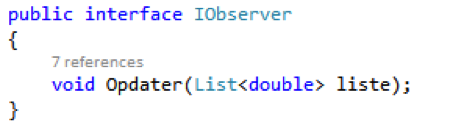
\includegraphics[width=0.7\textwidth]{Figurer/SoftwareImplementering/observer2}
	\caption{Interface IObserver. Subject sørger for at kalde metoden "Opdater()"\ for alle dens abonnenter}
	\label{observer2}
\end{figure}

\begin{figure}[H]
	\centering
	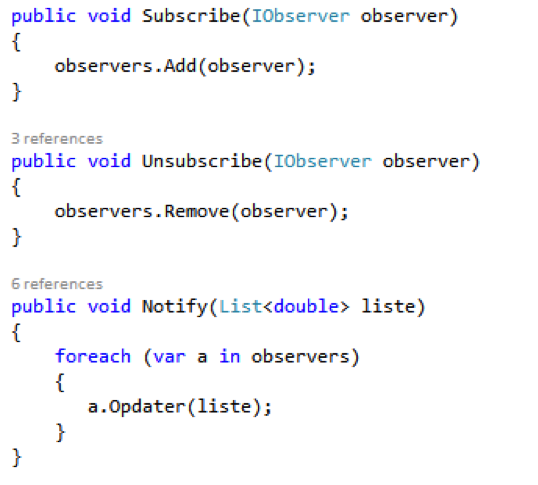
\includegraphics[width=0.7\textwidth]{Figurer/SoftwareImplementering/observer3}
	\caption{Implementeringen af subject-metoderne i Logik-klassen}
	\label{observer3}
\end{figure}
Der er anvendt push-metode, hvilket vil sige, at subject sender sin data med som parameter i Notify().\\
Observer-mønstret har vist sig nyttigt, da vi dermed undgår, at observers hele tiden skal tjekke, om der er kommet ny data. Dette sparer computerkræfter, hvilket er en nødvendighed, da mange af de opståede problemer er opstået på baggrund af, at computeren ikke har kunnet arbejde hurtigt nok.

\subsection{UML klassediagram}\label{UML klassediagram}
I dette afsnit ses et samlet og opdateret UML klassediagram over koden. 


\subsection{Kode udsnit}
I dette afsnit vil der være udsnit af det vigtigste og mest interessante kode. Der vil ligeledes være en beskrivelse af, hvilken funktion koden har.

\subsection{Diagrammer}
I dette afsnit vil udvalgte metoder i koden beskrives ud fra skevensdiagrammer og aktivitetsdiagrammer. Dette vil danne et systemisk overblik over hvordan metoderne i koden fungerer. 

 







